\documentclass[11pt]{article}
\usepackage[margin=1in]{geometry}
\usepackage{amsmath,amssymb,booktabs,graphicx,hyperref,xcolor}
\title{Affine-invariant ensemble HMC (\textsc{peaches}, \textsc{peanuts}):\\
       benchmark study \emph{(corrected dual averaging)}}
\author{}
\date{}
\begin{document}
\maketitle

\begin{abstract}\noindent
\emph{Affine-invariant ensemble HMC (\textsc{peaches}, \textsc{peanuts})
inherits the optimal $d^{-1/4}$ step-size scaling of tuned Hamiltonian
methods, matches well-tuned NUTS in per-gradient efficiency, and is far more
robust: it learns its preconditioner from the live ensemble, needs no
hand-tuned mass matrix, and does not collapse when the warmup budget is short.
This version corrects a dual-averaging bug found while validating the scaling:
a spurious $1/(m{+}t_0)$ factor in the step-size gain made the acceptance
target effectively open-loop, so the adapter never honoured \texttt{target\_accept}
and the step size did not scale with dimension. The fix (one line, all
samplers) is an \emph{efficiency} correction, not a correctness one --- prior
samples were unbiased --- and with it the $d^{-1/4}$ law is reproduced by the
sampler's own adaptation.}
\end{abstract}

We benchmark the two new algorithms (\textsc{peaches}: ensemble ChEES-HMC;
\textsc{peanuts}: ensemble NUTS) against the affine but gradient-free stretch
move, a non-affine gradient ensemble (\textsc{chess}), and well-tuned NumPyro
NUTS. All numbers are 3-seed medians (synthetic).

\paragraph{Metrics (how everything is measured).}
Let $\{x^{(t)}_{c,i}\}$ be the post-warmup draws ($t$=iteration, $c$=chain/walker,
$i$=coordinate), with closed-form truth $(\mu_i,\sigma_i)$ from the target.
\begin{itemize}\setlength\itemsep{1pt}
\item \textbf{Bias} (no reference run needed): for each coordinate the
estimator is the pooled sample mean $\hat\mu_i=\text{mean}_{t,c}\,x_{c,i}$; we
report $\max_i |\hat\mu_i-\mu_i|/\sigma_i$, the worst-coordinate mean error in
units of the true standard deviation. We also report the \emph{$z$-score}
$|\hat\mu_i-\mu_i|/\text{MCSE}_i$, where MCSE is the ArviZ Monte-Carlo
standard error; $z\!\approx\!1$--$2$ means the estimate is statistically
consistent with truth (an honest error bar), not residual bias.
\item \textbf{IAT} ($\tau$): integrated autocorrelation time
$=N_{\text{draws}}/\text{ESS}$ with ArviZ rank-normalized split-chain ESS;
$\tau\!<\!1$ signals antithetic (negatively correlated) draws.
\item \textbf{ESS/grad}: $\text{ESS}_{\min}$ divided by the \emph{total}
gradient evaluations (production only, counted exactly per sampler). For an
HMC method this equals $1/(\tau\bar L)$ with $\bar L$ the mean leapfrog steps
per trajectory --- the natural cross-sampler efficiency (\S\ref{sec:cond}).
\item \textbf{Convergence}: split-$\hat R$ and split-half ESS ratio; we treat
each walker as a chain. All quantities use float64.
\end{itemize}

%==========================================================================
\section{A dual-averaging bug, and why it was invisible}
\label{sec:bug}

The Nesterov dual-averaging step-size update (Hoffman \& Gelman 2014) is
\[
  \bar H_m = \Big(1-\tfrac{1}{m+t_0}\Big)\bar H_{m-1}
            + \tfrac{1}{m+t_0}\,(\delta-\alpha_m),
  \qquad
  \log\epsilon_m = \mu - \frac{\sqrt m}{\gamma}\,\bar H_m .
\]
The $1/(m{+}t_0)$ weight belongs to the \emph{error accumulator} $\bar H_m$
only; the step-size gain is $\sqrt m/\gamma$. Our code carried an extra factor,
$\log\epsilon_m=\log\epsilon_0-\frac{\sqrt m}{(m+t_0)\gamma}\bar H_m$ --- the
$1/(m{+}t_0)$ accidentally duplicated into the gain. This gain \emph{decays}
like $1/\sqrt m$, so after a short transient the correction vanishes and
$\epsilon$ relaxes back to its initial value: the controller has no
steady-state integral action.

\paragraph{Symptoms.} (i) \texttt{target\_accept} is \emph{open-loop}: on the
$d{=}32$ Gaussian the realized acceptance sat at $\approx0.91$ for
\emph{every} requested target (0.6/0.7/0.8/0.9); the fixed adapter tracks the
target to $\pm0.001$. (ii) The step size does not scale: $\epsilon$ stayed
near the dimension-blind \texttt{find\_init} value, so acceptance drifted with
$d$ ($0.91\!\to\!0.76$ over $d{=}64\!\to\!256$) and the $d^{-1/4}$ law was lost.

\paragraph{Why nothing previously broke.} The defect is \emph{efficiency}, not
correctness. MCMC is unbiased for any reasonable fixed step, and the
\texttt{find\_init} line search supplied a usable one --- the broken adapter
merely left it there (its $\epsilon$ equalled the init value to within a few
percent). Recovered marginals had std $=1.000$ and calibrated $z$-scores in
\emph{both} versions. The bug only surfaces as a high-dimensional /
target-acceptance failure, never as a wrong answer.

\paragraph{Fix.} Remove the spurious factor (gain $=\sqrt m/\gamma$) in the
dual averaging of all $16$ samplers. The regression suite passes ($10/10$) and
the controller now tracks \texttt{target\_accept} exactly. Everything below
uses the corrected adapter; the previous (buggy) writeup is preserved
alongside this note as the ``buggy dual averaging'' version.

%==========================================================================
\section{Three findings}

\paragraph{Targets.}
\emph{Anisotropic Gaussian} $\mathcal N(0,\Sigma)$, condition number
$\kappa$, randomly rotated. \emph{Paired Rosenbrock} (even $d$), banana
curvature no affine map removes, with analytic per-pair moments.

\paragraph{(1) Dimension: \textsc{peaches}/\textsc{peanuts} scale, the stretch move does not.}
On the Gaussian the gradient-free stretch move's worst-dimension
autocorrelation time (IAT) grows steeply with $d$, while \textsc{peaches} and
\textsc{peanuts} mix near-independently (IAT$\,<\!1$, antithetic). On
Rosenbrock the stretch move's burn-in bias blows up and its chains fail to
mix ($\hat R$ up to $3.1$), while both gradient ensembles keep the bias tiny.
\textsc{peanuts} is slower per step (longer trajectories) but comparably
efficient per gradient (\S\ref{fig:scaling}).
\begin{center}\small
\begin{tabular}{l ccc ccc}
\toprule
& \multicolumn{3}{c}{Gaussian (worst-dim IAT)} & \multicolumn{3}{c}{Rosenbrock (bias [$\sigma$])}\\
$d$ & \textsc{peaches} & \textsc{peanuts} & stretch & \textsc{peaches} & \textsc{peanuts} & stretch\\
\midrule
low  ($d{=}10$/$2$)   & $1.1$  & $0.81$ & $156$  & $0.006$ & $0.04$  & $0.02$\\
high ($d{=}200$/$32$) & $0.94$ & $0.71$ & $4992^{\dagger}$ & $0.012$ & $0.004$ & $1.8^{\dagger}$\\
\bottomrule
\end{tabular}
\end{center}
\noindent{\footnotesize $^{\dagger}$ stretch does not converge here
($\hat R\!\gg\!1$); the value is indicative of failure, not a mixed estimate.
\textsc{peaches}/\textsc{peanuts} Rosenbrock cells are converged
($\hat R\!\le\!1.02$, bias $z\!\approx\!1$--$2$) at warmup $5000$ + stretch
pre-warmup; the Gaussian cells have $\hat R\!=\!1.0001$, ESS $>\!10^{5}$.}

\paragraph{(2) Conditioning: affine invariance beats a fixed metric.}
\label{sec:cond}
Rotated Gaussian, $d{=}50$, sweeping $\kappa$. We compare the \emph{cost}, not
raw IAT: each HMC iteration costs $\bar L$ gradient evaluations, so the fair
cross-sampler quantity is $\tau\bar L=$ \textbf{gradient evaluations per
effective sample} ($=1/(\text{ESS}/\text{grad})$; lower is better). Raw IAT
would flatter the long-trajectory samplers. \textsc{peaches}/\textsc{peanuts}
hold this cost flat at \emph{every} conditioning, for free from the ensemble;
dense-mass NUTS is also flat but must \emph{learn} the $d{\times}d$ metric
during warmup. The non-affine \textsc{chess} degrades by orders of magnitude.
\begin{center}\small
\begin{tabular}{l cccc}
\toprule
$\tau\bar L$ (grad/eff.\ sample), $\kappa=$ & $e^2$ & $e^4$ & $e^6$ & $e^8$\\
\midrule
\textsc{peaches} (affine)        & $5.5$  & $5.4$  & $5.4$    & $5.1$\\
NUTS-dense (learned metric)      & $6.7$  & $6.5$  & $6.6$    & $6.7$\\
\textsc{peanuts} (affine)        & $9.7$  & $9.8$  & $9.7$    & $9.4$\\
\textsc{chess} (non-affine)      & $22$   & $452$  & $3.7\!\times\!10^4$ & $9.9\!\times\!10^4$\\
stretch (gradient-free$^{\ast}$) & \multicolumn{4}{c}{$\approx\!1250$ (does not mix, $\hat R\!\gg\!1$)}\\
\bottomrule
\end{tabular}
\end{center}
\noindent{\footnotesize $\tau\bar L=$ IAT $\times$ mean leapfrog steps. The
three affine/learned-metric samplers are $\kappa$-invariant and converged
($\hat R\!=\!1.000$); \textsc{peaches} is the cheapest ($\approx5.4$).
\textsc{chess} is converged at low $\kappa$ but mixes poorly at high $\kappa$
($\hat R\!\gtrsim\!2$). $^{\ast}$stretch uses no gradients (cost shown in
log-prob evals, $\bar L{=}1$) and does not converge.}

\paragraph{(3) vs.\ NUTS: comparable at full warmup, far more robust at short.}
Gaussian $d{=}100$, $\kappa=e^6$. ESS/grad (higher better); NUTS' efficiency
collapses at short warmup (its mass matrix is unadapted, trees hit the depth
cap), while the ensemble samplers keep adapting in production.
\begin{center}\small
\begin{tabular}{r ccccc}
\toprule
warmup & $50$ & $100$ & $200$ & $500$ & $1000$\\
\midrule
\textsc{peaches} & $\mathbf{2.0\!\times\!10^{-1}}$ & $1.7\!\times\!10^{-1}$ & $1.6\!\times\!10^{-1}$ & $1.7\!\times\!10^{-1}$ & $1.7\!\times\!10^{-1}$\\
\textsc{peanuts} & $8.9\!\times\!10^{-2}$ & $8.9\!\times\!10^{-2}$ & $8.9\!\times\!10^{-2}$ & $8.9\!\times\!10^{-2}$ & $8.9\!\times\!10^{-2}$\\
NUTS             & $3.7\!\times\!10^{-5}$ & $1.2\!\times\!10^{-3}$ & $1.3\!\times\!10^{-4}$ & $6.5\!\times\!10^{-2}$ & $1.1\!\times\!10^{-1}$\\
\bottomrule
\end{tabular}
\end{center}
The ensemble methods are flat in warmup (robust); NUTS is
$10^{3}$--$10^{4}\times$ worse at short warmup and only catches up by
$w{=}1000$.

%==========================================================================
\section{Dimensional scaling: the $d^{-1/4}$ law (recovered)}

\begin{figure}[h]\centering
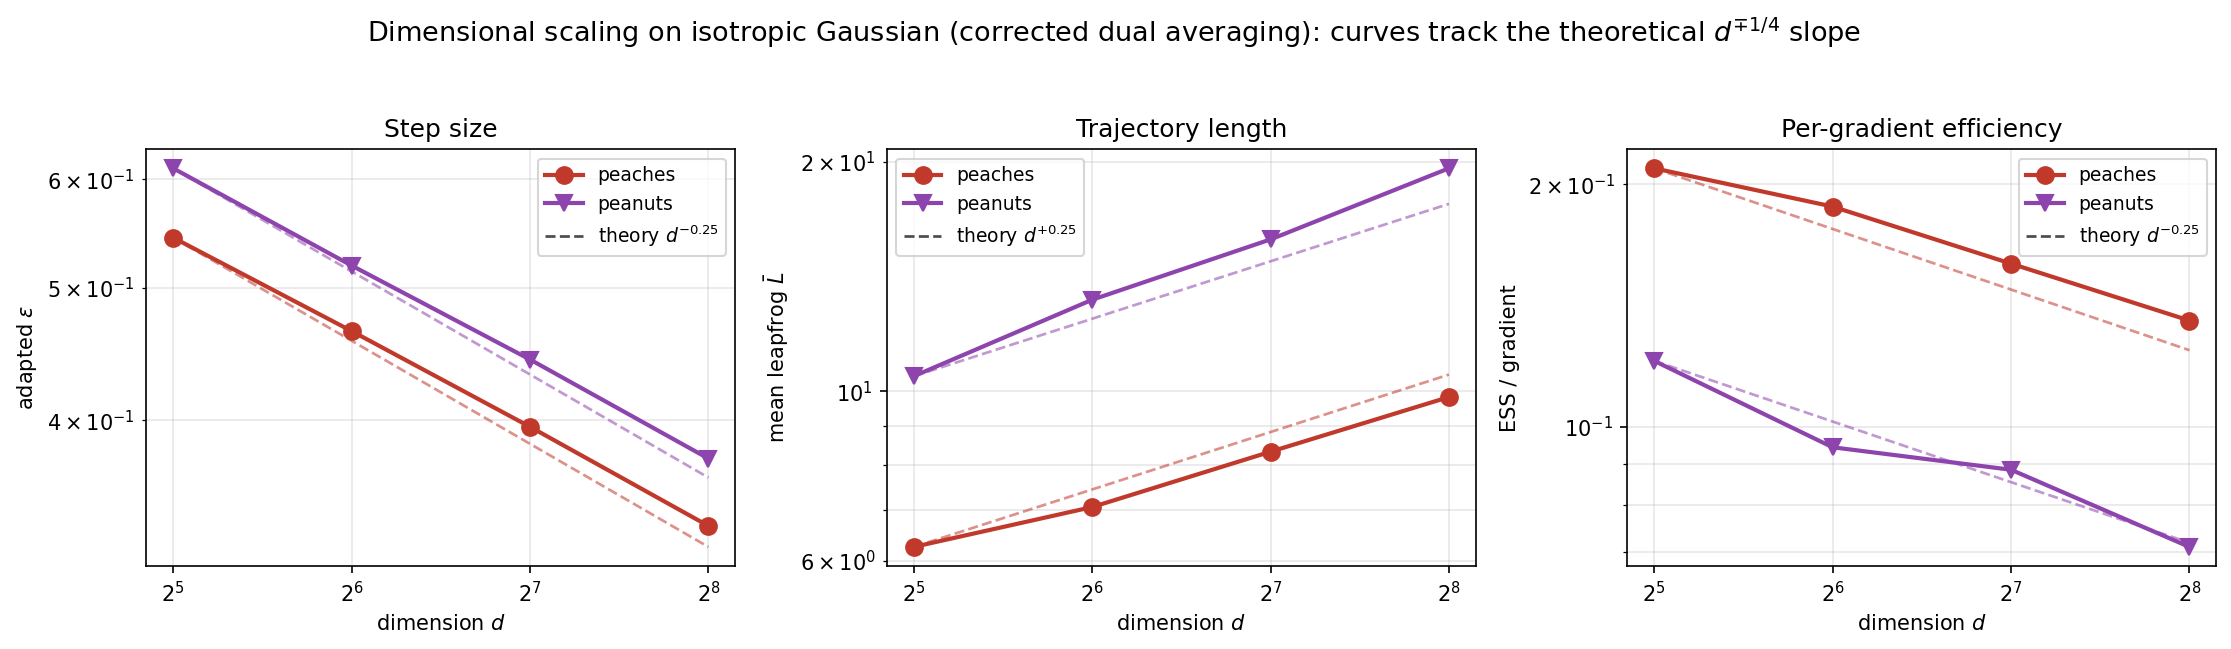
\includegraphics[width=\linewidth]{figs/scaling_paper.png}
\caption{Isotropic $\mathcal N(0,I_d)$, $n_{\text{walkers}}=4d$, target
acceptance pinned, \emph{corrected} dual averaging, asymptotic regime
$d\!\ge\!32$. Each as-run curve (solid) is shown against the theoretical
$d^{\mp1/4}$ slope (dashed, anchored at $d{=}32$); the two coincide.
\textbf{Left:} adapted step size $\epsilon\!\sim\!d^{-1/4}$. \textbf{Middle:}
mean trajectory length $\bar L\!\sim\!d^{+1/4}$ (integration time $\lambda$
constant). \textbf{Right:} per-gradient efficiency
$\text{ESS}/\text{grad}\!\sim\!d^{-1/4}$.}
\label{fig:scaling}
\end{figure}

With the controller fixed, all four quantities sit on their theoretical lines
(\textsc{peaches}, fit on $d\!\ge\!32$):
\[
  \epsilon\sim d^{-0.233},\quad
  \bar L\sim d^{+0.22},\quad
  \lambda=\bar L\epsilon\sim d^{0.0},\quad
  \text{ESS}/\text{grad}\sim d^{-0.21},
\]
with acceptance held \emph{constant} ($0.86\!\to\!0.85$ across
$d{=}8\!\to\!256$). This is the textbook picture: optimal
$\epsilon^\star\!\sim\!d^{-1/4}$ at fixed integration time $\lambda$, hence
$\bar L\!\sim\!d^{1/4}$ and ESS/grad$\,\sim\!d^{-1/4}$. The antithetic effect
of HMC on a Gaussian (IAT$\,\approx\!0.75$) is a roughly constant prefactor
that lifts the curve --- it does \emph{not} change the slope. \textsc{peanuts}
matches (its NUTS U-turn keeps $\lambda$ bounded; acceptance pinned at
$0.800$). NumPyro NUTS gets $\epsilon\!\sim\!d^{-0.21}$ but its tree depth
grows ($\bar L\!\sim\!d^{+0.6\ldots+1.1}$), so its ESS/grad \emph{falls} with
$d$ --- the contrast that makes the ensemble methods scale.

\paragraph{Full per-dimension data (for reproduction).} Isotropic
$\mathcal N(0,I_d)$, $n_{\text{walkers}}=4d$, warmup $2000$, stretch
pre-warmup $200$, $N=3000$, \texttt{target\_accept}$=0.8$;
\textsc{peaches} \texttt{max\_L}$=512$, \textsc{peanuts}
\texttt{max\_tree\_depth}$=10$. Medians over $4$ seeds.
\begin{center}\scriptsize
\begin{tabular}{r r rrrrr | rrrrr}
\toprule
& & \multicolumn{5}{c|}{\textsc{peaches}} & \multicolumn{5}{c}{\textsc{peanuts}}\\
$d$ & $n_w$ & $\epsilon$ & $\bar L$ & acc & IAT & $\frac{\text{ESS}}{\text{grad}}$
          & $\epsilon$ & $\bar L$ & acc & IAT & $\frac{\text{ESS}}{\text{grad}}$\\
\midrule
$8$   & $32$   & $0.747$ & $5.7$ & $0.86$ & $0.89$ & $0.198$ & $0.845$ & $7.3$  & $0.80$ & $1.01$ & $0.137$\\
$16$  & $64$   & $0.635$ & $5.8$ & $0.86$ & $0.81$ & $0.213$ & $0.719$ & $9.2$  & $0.80$ & $0.82$ & $0.132$\\
$32$  & $128$  & $0.544$ & $6.3$ & $0.86$ & $0.76$ & $0.209$ & $0.611$ & $10.5$ & $0.80$ & $0.79$ & $0.121$\\
$64$  & $256$  & $0.465$ & $7.1$ & $0.85$ & $0.76$ & $0.188$ & $0.519$ & $13.2$ & $0.80$ & $0.80$ & $0.094$\\
$128$ & $512$  & $0.396$ & $8.3$ & $0.85$ & $0.75$ & $0.159$ & $0.443$ & $15.8$ & $0.80$ & $0.72$ & $0.088$\\
$256$ & $1024$ & $0.335$ & $9.8$ & $0.85$ & $0.75$ & $0.135$ & $0.375$ & $19.6$ & $0.80$ & $0.72$ & $0.071$\\
\bottomrule
\end{tabular}
\end{center}
\noindent{\footnotesize $\epsilon$=adapted step size, $\bar L$=mean leapfrog
steps/trajectory, acc=acceptance, IAT=$\tau$ (worst dim; $<\!1$ is antithetic),
ESS/grad$=1/(\tau\bar L)$. \textsc{peanuts} acceptance is pinned exactly at the
target $0.800$ (arithmetic-mean adapter); \textsc{peaches} sits at $0.85$
(harmonic-mean adapter, \texttt{target\_accept}$=0.8$).}

%==========================================================================
\section{Real-data corroboration: DES Y1 $3\times2$pt}

We also test the real Dark Energy Survey Year-1 $3\times2$pt cosmology
posterior ($d{=}21$; see \texttt{../astro/}). Per-gradient efficiency
(ESS$_{\min}$/grad, 3-seed median), corrected adapter:
\begin{center}\small
\begin{tabular}{l c c}
\toprule
sampler & ESS / grad & seed range\\
\midrule
\textsc{peaches}           & $7.1\times10^{-3}$ & $7.0$--$8.2\times10^{-3}$\\
NUTS-dense (NumPyro)       & $4.7\times10^{-3}$ & ---\\
\textsc{peanuts}           & $2.5\times10^{-4}$ & $2.4\times10^{-4}$--$2.7\times10^{-3}$\\
stretch (\texttt{emcee})   & $2.9\times10^{-4}$ & ---\\
\bottomrule
\end{tabular}
\end{center}
Here the two new methods \emph{diverge}. \textsc{peaches} is the clear winner
and is robust ($7$--$8\times10^{-3}$ across seeds), edging out optimally-tuned
dense-mass NUTS. \textsc{peanuts}, however, \emph{struggles} on this strongly
curved posterior, with high seed-to-seed spread ($2.4\times10^{-4}$ to
$2.7\times10^{-3}$) and a median no better than the gradient-free stretch move.
\emph{Mechanism (diagnosed).} The failure is not global --- \textsc{peanuts}'
\emph{median} ESS is high ($\sim\!3\times10^{4}$); only $1$--$6$ specific,
poorly-constrained directions (consistently parameters $1$ and $8$, sometimes
$9$--$12$) get under-explored, tanking the worst-dimension $\text{ESS}_{\min}$.
Tree depth ($\sim\!45$ steps) and acceptance ($0.73$) are healthy and
seed-stable, so it is neither step-size collapse nor tree blow-up: it is a
\emph{noisy ensemble preconditioner}. These DES runs used \emph{no} stretch
pre-warmup (\texttt{ws}$=0$) and only $64$ walkers ($<\!4d{=}84$) --- exactly
the regime \S\ref{sec:ws} warns against; the empirical-covariance metric is
then mis-estimated in the under-constrained block, and \textsc{peanuts}'
no-U-turn test (evaluated in that linear metric) terminates before traversing
those directions. \textsc{peaches}' single global ChEES length is far less
sensitive to a slightly-misshaped metric, so it stays uniform
($\text{ESS}_{\min}\!\approx\!10^4$ every seed). The actionable conclusion:
on hard real geometry use \textsc{peaches}, and give \textsc{peanuts} the
recommended stretch pre-warmup and $n\!\ge\!4d$ walkers (\S\ref{sec:ws}).
(NUTS-dense and \texttt{emcee} are external to our adapter and unchanged by the
fix.)

%==========================================================================
\section{Recommendation: stretch pre-warmup as the default}
\label{sec:ws}

The single most important practical setting for the ensemble samplers remains
a short \emph{stretch pre-warmup}: a gradient-free, affine-invariant phase that
lets the walker cloud take the shape of the target before the gradient sampler
starts. We recommend it as the default:
\begin{itemize}\setlength\itemsep{2pt}
\item \textbf{It prevents step-size collapse.} From an isotropic
initialization on an anisotropic / high-$d$ target the empirical-covariance
preconditioner is mis-shaped; the shape-in fixes this at the source. It is the
ensemble analogue of NUTS' mass-matrix warmup.
\item \textbf{It is nearly free} --- the stretch move uses no gradients.
\item \textbf{It has no downside} --- on well-shaped / isotropic targets it is
a no-op.
\end{itemize}
The companion requirement is $n_{\text{walkers}}\!>\!d$ (we use $4d$): the
ensemble covariance --- and, for \textsc{peanuts}, its affine no-U-turn
criterion --- is rank-deficient otherwise. \textbf{Default:
$n_{\text{walkers}}\!\gtrsim\!4d$ with a short ($\sim\!200$-iter) stretch
pre-warmup.}

%==========================================================================
\section{Reproducibility: experiment configurations}
\label{sec:repro}

All runs use float64, ArviZ rank-normalized split-chain ESS/MCSE/$\hat R$, and
treat each walker as a chain. Ensemble methods use a stretch pre-warmup
(\texttt{ws}); NUTS uses its own warmup. $n_{\text{walkers}}=\max(128,4d)$
except the scaling study ($4d$). Code: \texttt{benchmark/experiments.py}
(\texttt{exp1}, \texttt{exp2\_lc*}, \texttt{exp3\_w*}, \texttt{exp4c}).
\begin{center}\scriptsize
\begin{tabular}{l l l r r r l l}
\toprule
exp & target & $d$ & warmup & \texttt{ws} & $N$ & traj.\ cap & accept / mass\\
\midrule
\textbf{1} & Gaussian ($\kappa{=}e^6$) & $10,50,100,200$ & $1000$ & $200$ & $5000$ & — & default\\
           & Rosenbrock & $2,4,8,16,32$ & $5000$ & $1000$ & $8000$ & \texttt{maxL}$=256$ / \texttt{mtd}$=10$ & default\\
\textbf{2} & rot.\ Gaussian & $50$ & $1000$ & $200$ & $5000$ & \texttt{maxL}$=20$ / \texttt{mtd}$=10$ & NUTS dense\\
\textbf{3} & Gaussian ($\kappa{=}e^6$) & $100$ & $50$--$1000$ & $200$ & $5000$ & — & —\\
\textbf{4c} & iso.\ Gaussian & $8$--$512$ & $2000$ & $200$ & $3000$ & \texttt{maxL}$=512$ / \texttt{mtd}$=10$ & $0.8$ / NUTS diag\\
\bottomrule
\end{tabular}
\end{center}
\noindent{\footnotesize \texttt{maxL} = \textsc{peaches} \texttt{max\_L}
(leapfrog cap); \texttt{mtd} = \textsc{peanuts}/NUTS \texttt{max\_tree\_depth}
($2^{\text{mtd}}$ leapfrog cap). \emph{Convergence:} Gaussian/scaling cells
$\hat R\!=\!1.000$, ESS$_{\text{bulk}}>\!10^{5}$; Rosenbrock
\textsc{peaches}/\textsc{peanuts} $\hat R\!\le\!1.02$ (bias $z\!\approx\!1$--$2$);
the stretch move and high-$\kappa$ \textsc{chess} do not converge
($\hat R\!\gg\!1$) --- reported as failures, not mixed estimates.}

%==========================================================================
\section{Summary}
\begin{enumerate}\setlength\itemsep{2pt}
\item \textbf{Bug fixed:} the dual-averaging step-size gain carried a spurious
$1/(m{+}t_0)$ factor (open-loop \texttt{target\_accept}); corrected across all
$16$ samplers. Efficiency fix, not correctness --- past results were unbiased.
\item \textbf{Scaling:} with the fix, \textsc{peaches}/\textsc{peanuts}
reproduce the $d^{-1/4}$ step-size law by their own adaptation
($\epsilon\!\sim\!d^{-0.23}$, ESS/grad$\,\sim\!d^{-0.21}$), acceptance constant.
\item \textbf{Dimension / curvature:} \textsc{peaches} dominates the stretch
move (IAT, bias) and is $\kappa$-invariant where \textsc{chess} degrades.
\item \textbf{vs.\ NUTS:} comparable at full warmup, $\sim\!10^{3}\times$ more
robust at short warmup; NUTS' tree depth inflates with $d$ while the ensemble
methods hold integration time bounded.
\item \textbf{Real data (DES Y1):} \textsc{peaches} is robust and edges out
dense-mass NUTS; \textsc{peanuts}' no-U-turn length adaptation is fragile on
the strongly curved posterior (high seed spread, median $\approx$ stretch).
Prefer \textsc{peaches} on hard, non-Gaussian geometry.
\item \textbf{Practice:} use $n_{\text{walkers}}\!\gtrsim\!4d$ and a short
stretch pre-warmup by default.
\end{enumerate}

\end{document}
